%----------------------------------------------------------------------------------------
\begin{frame}
  \frametitle{TGV {\small Taylor-Green Vortex flow}}
  \only<1-2>{
  \textbf{Problem setting:}
  \begin{itemize}
    \itemsep-0.10cm
 	\item Prescribed initial condition
  	\item $Re=1600$
	\item Different mesh discretizations ($ Q_1/Q_1 $ and $ Q_2/Q_2 $)
  \end{itemize}
  \only<1>{
  	  \vspace*{-0.3cm}
	  \begin{figure}
	    \centering	
	    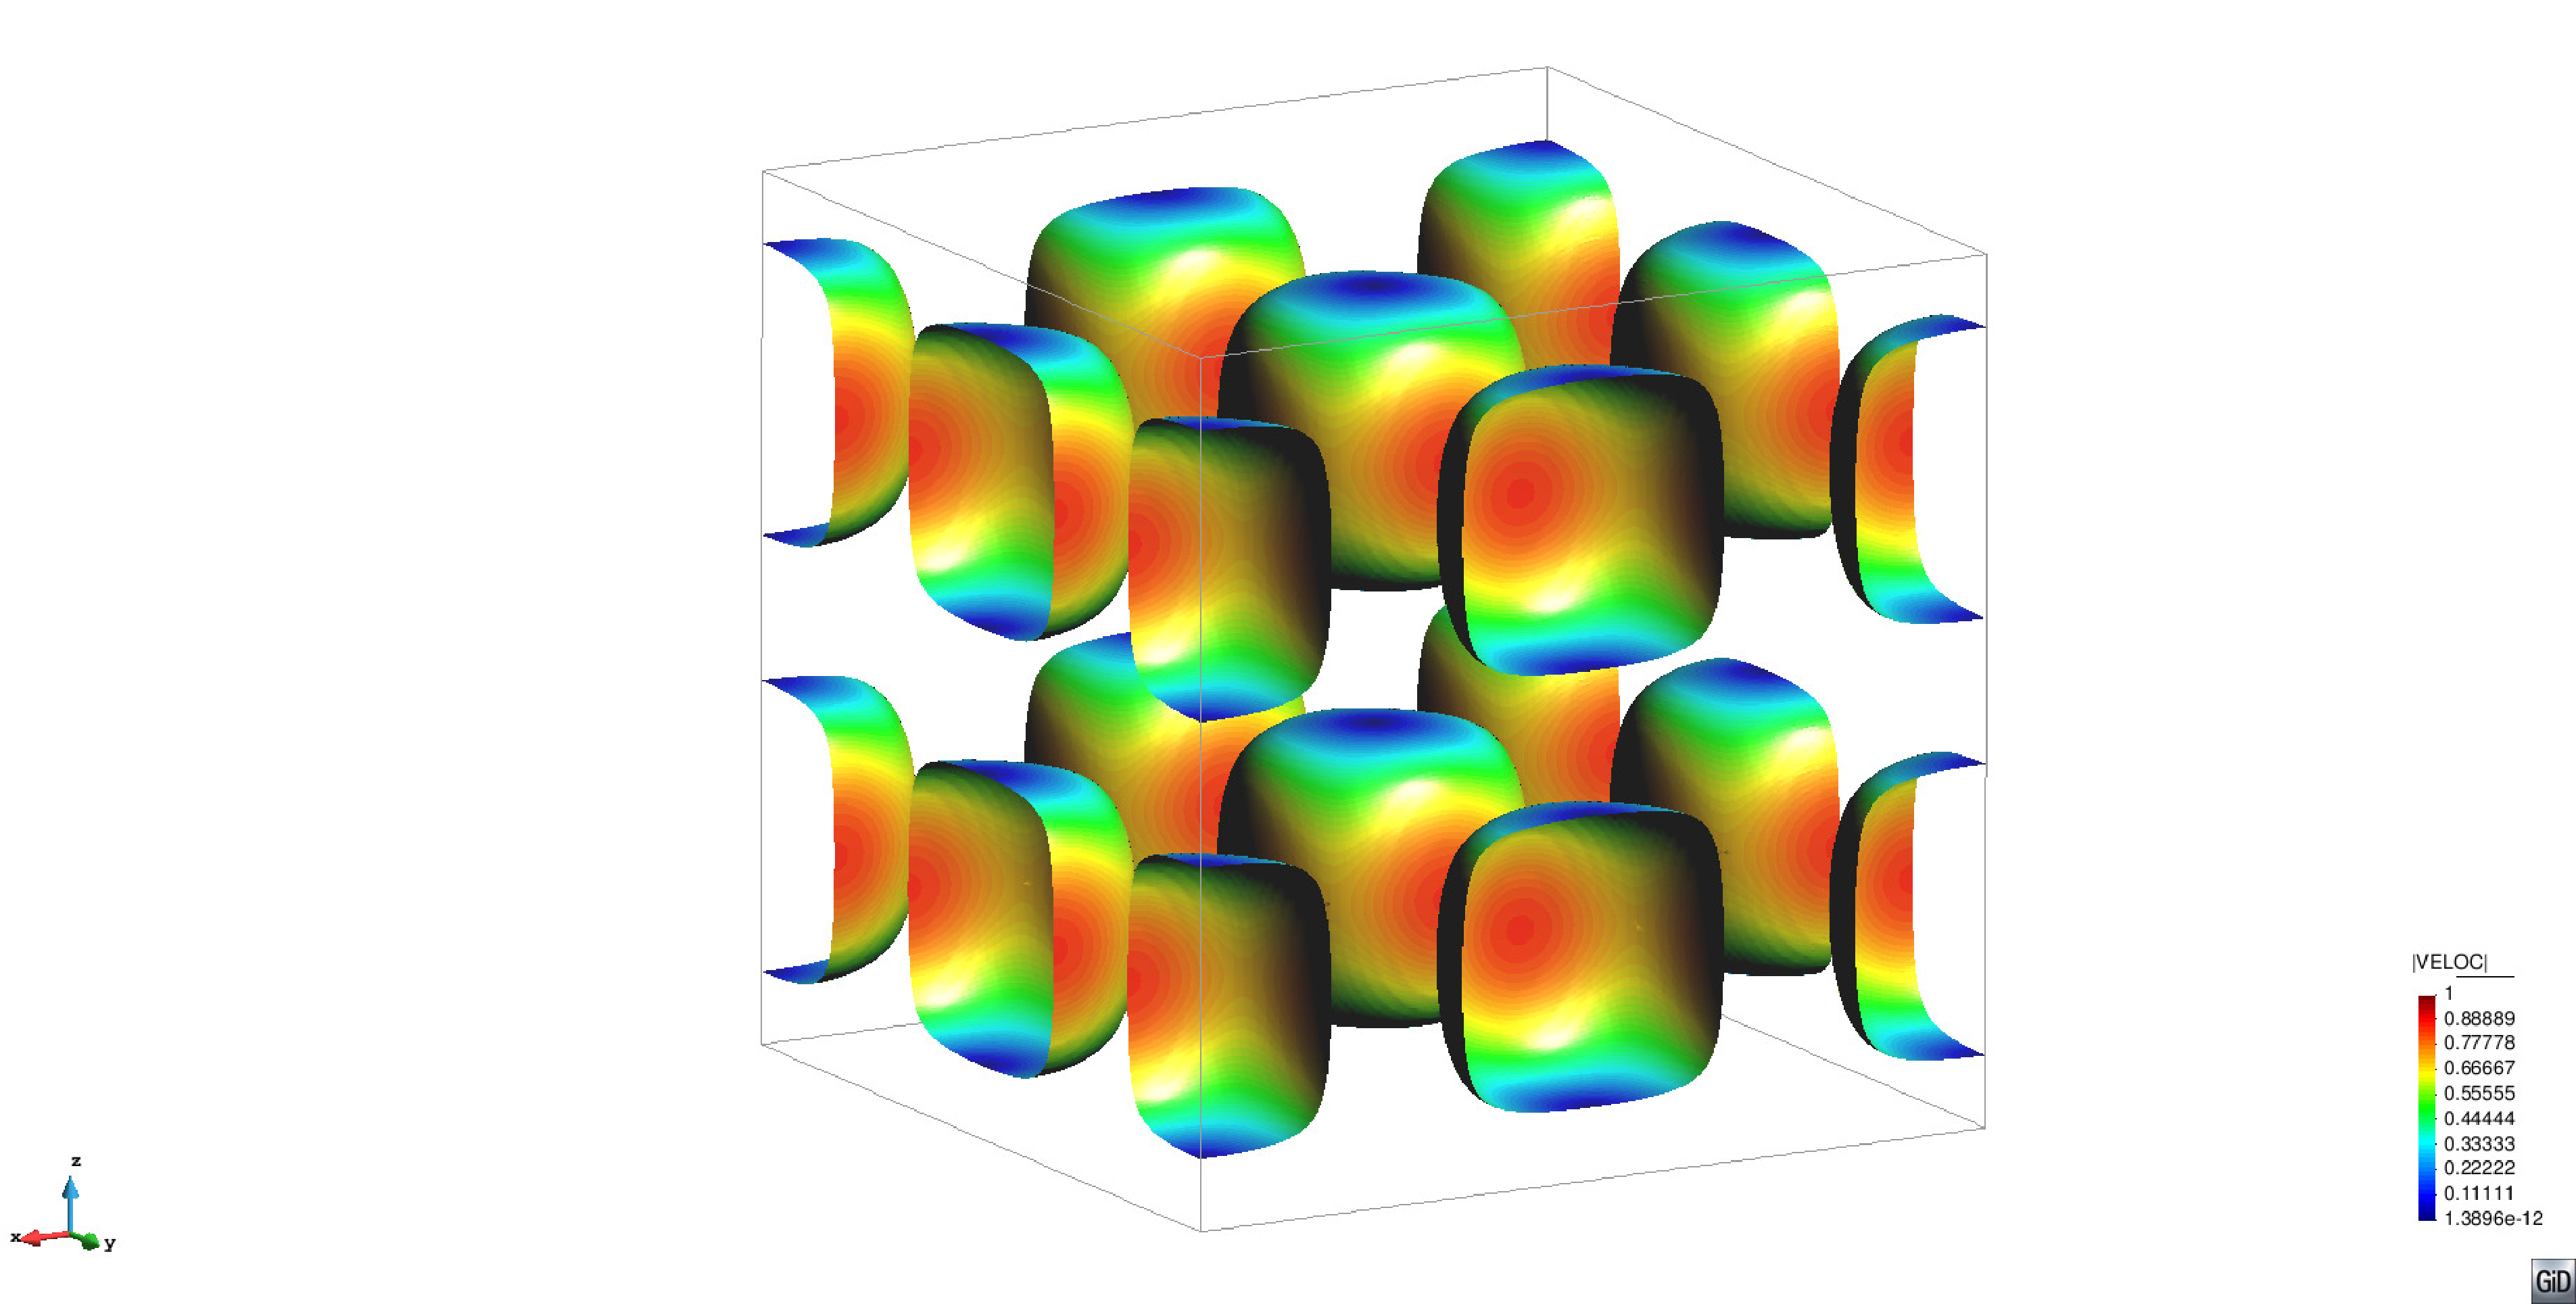
\includegraphics[trim=18cm 1cm 14cm 1cm, clip=true, width=0.45\textwidth]{Figures/isovorti_veloc_1.pdf}
	    \vspace*{-0.2cm}
	    \caption{Initial vorticity isosurface $|\omega|=1$}
	  \end{figure}}
  \only<2>{
      \vspace*{-0.3cm}
	  \begin{figure}
	    \centering	
	    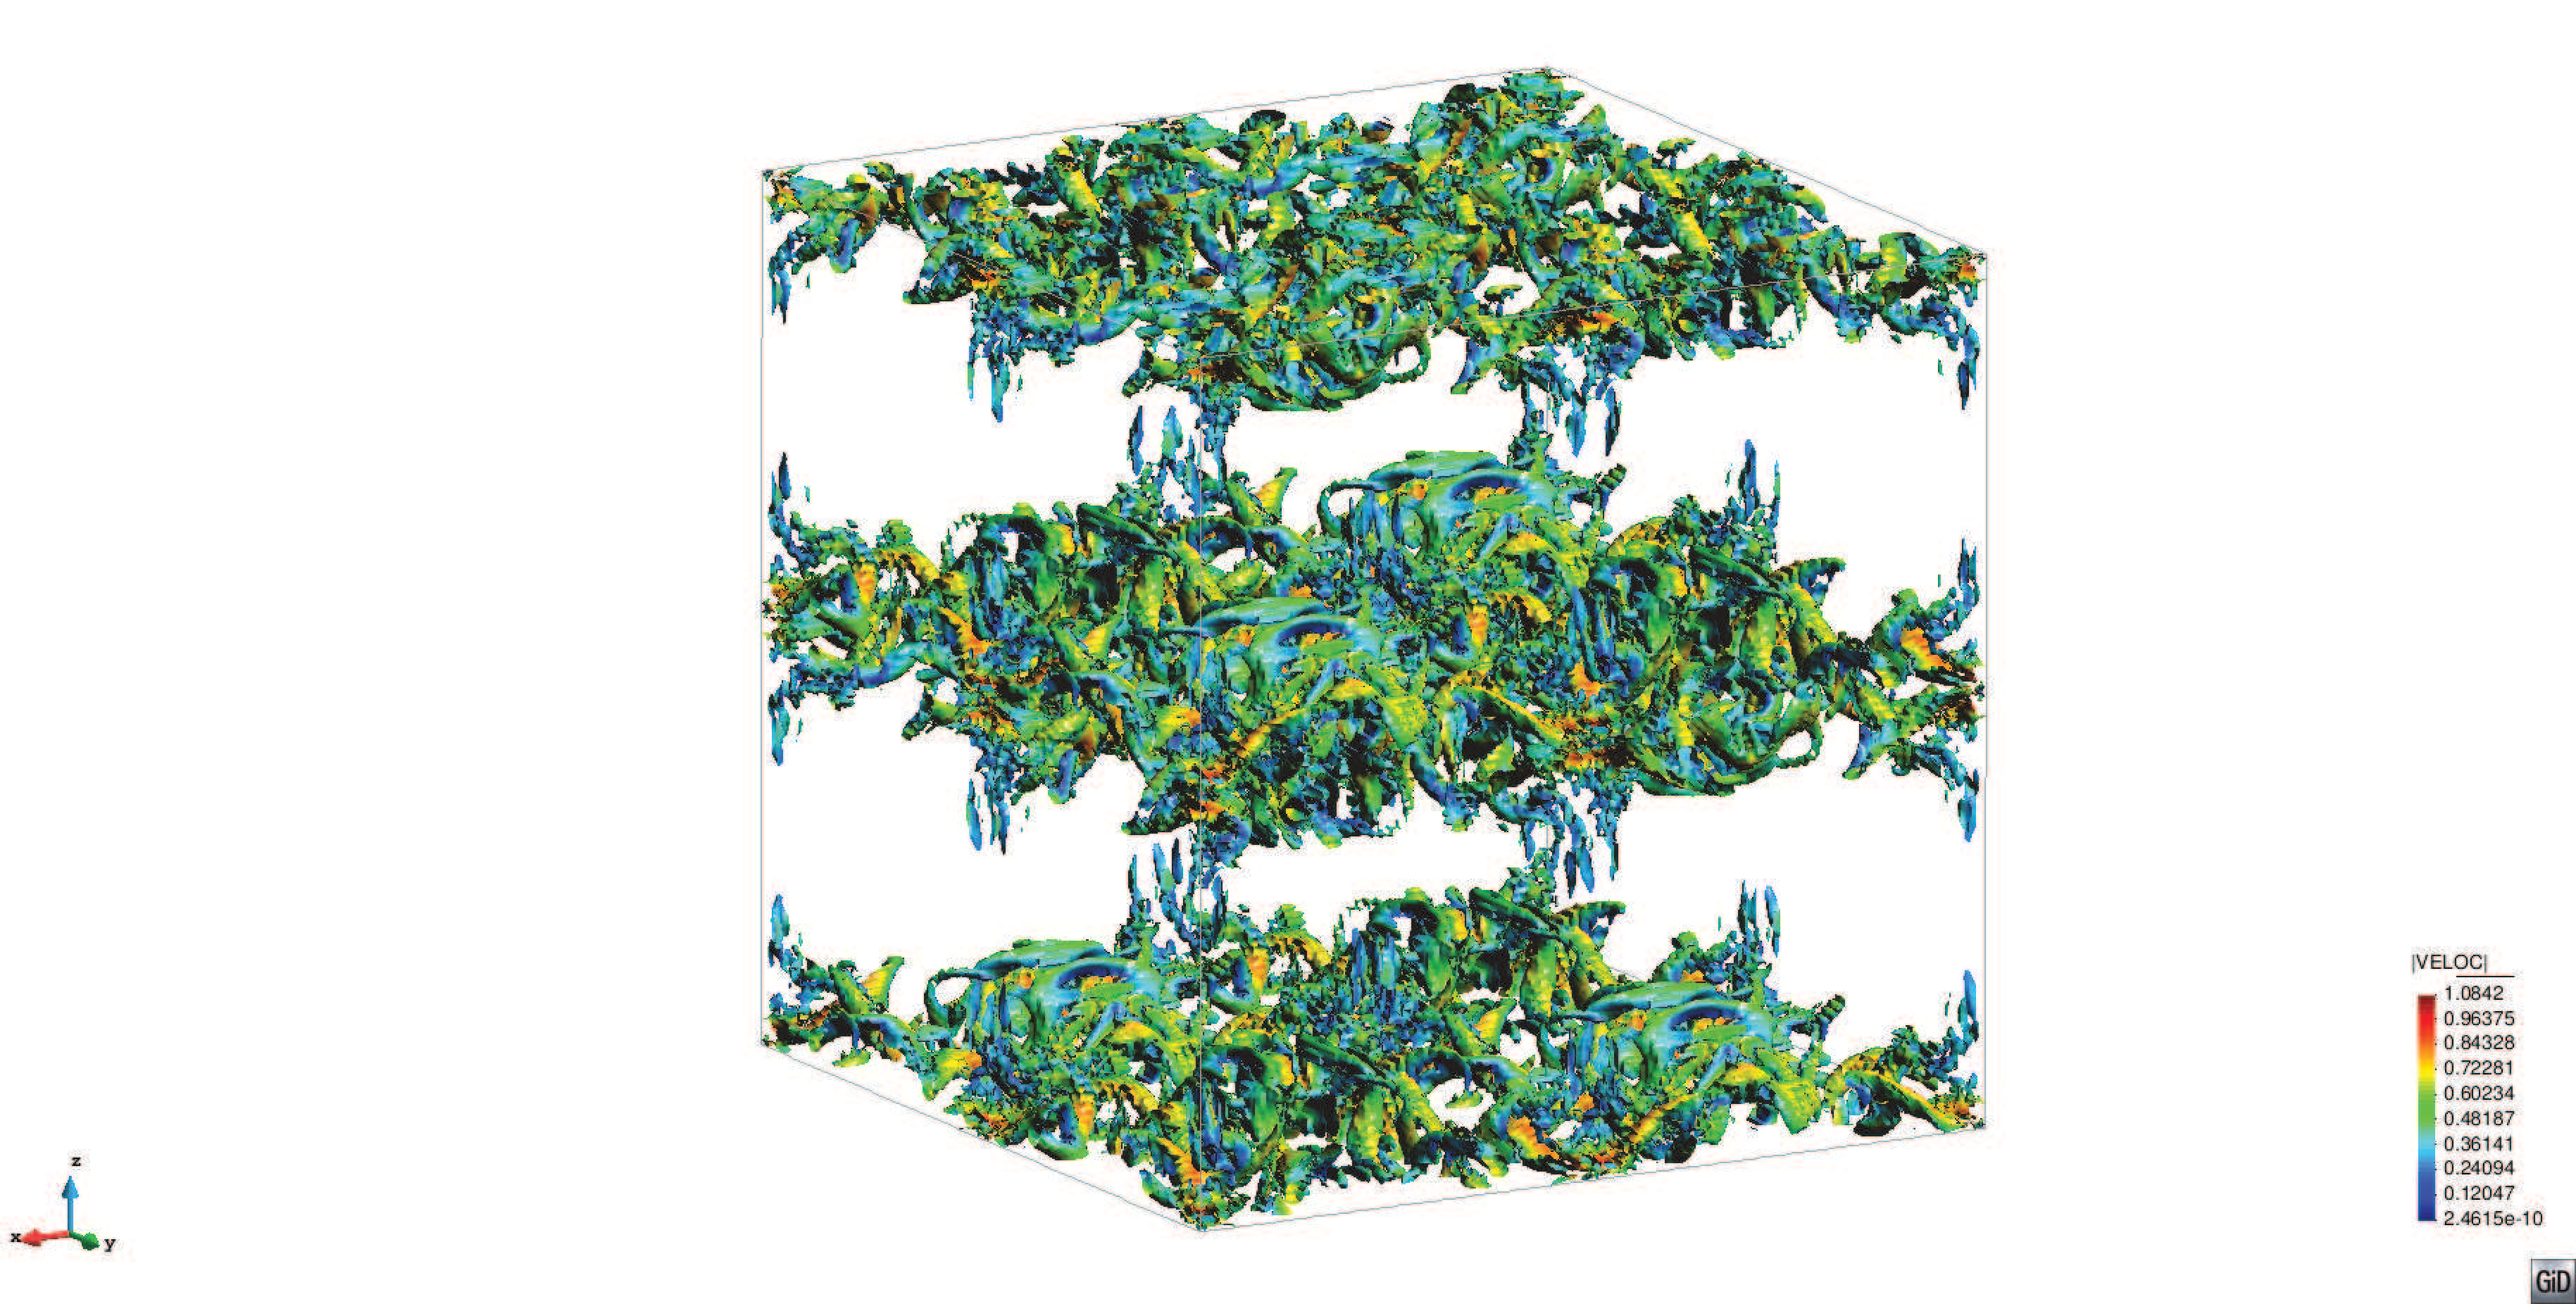
\includegraphics[trim=18cm 1cm 14cm 1cm, clip=true, width=0.45\textwidth]{Figures/isovorti_veloc_6.pdf}
	    \vspace*{-0.2cm}
	    \caption{Vorticity isosurfaces $|\omega|=9.0$}
	  \end{figure}}}
\only<3>{
\begin{figure}[h!]
\centering    
\movie[label=show3,width=1.0\textwidth,poster,autostart,showcontrols,loop]{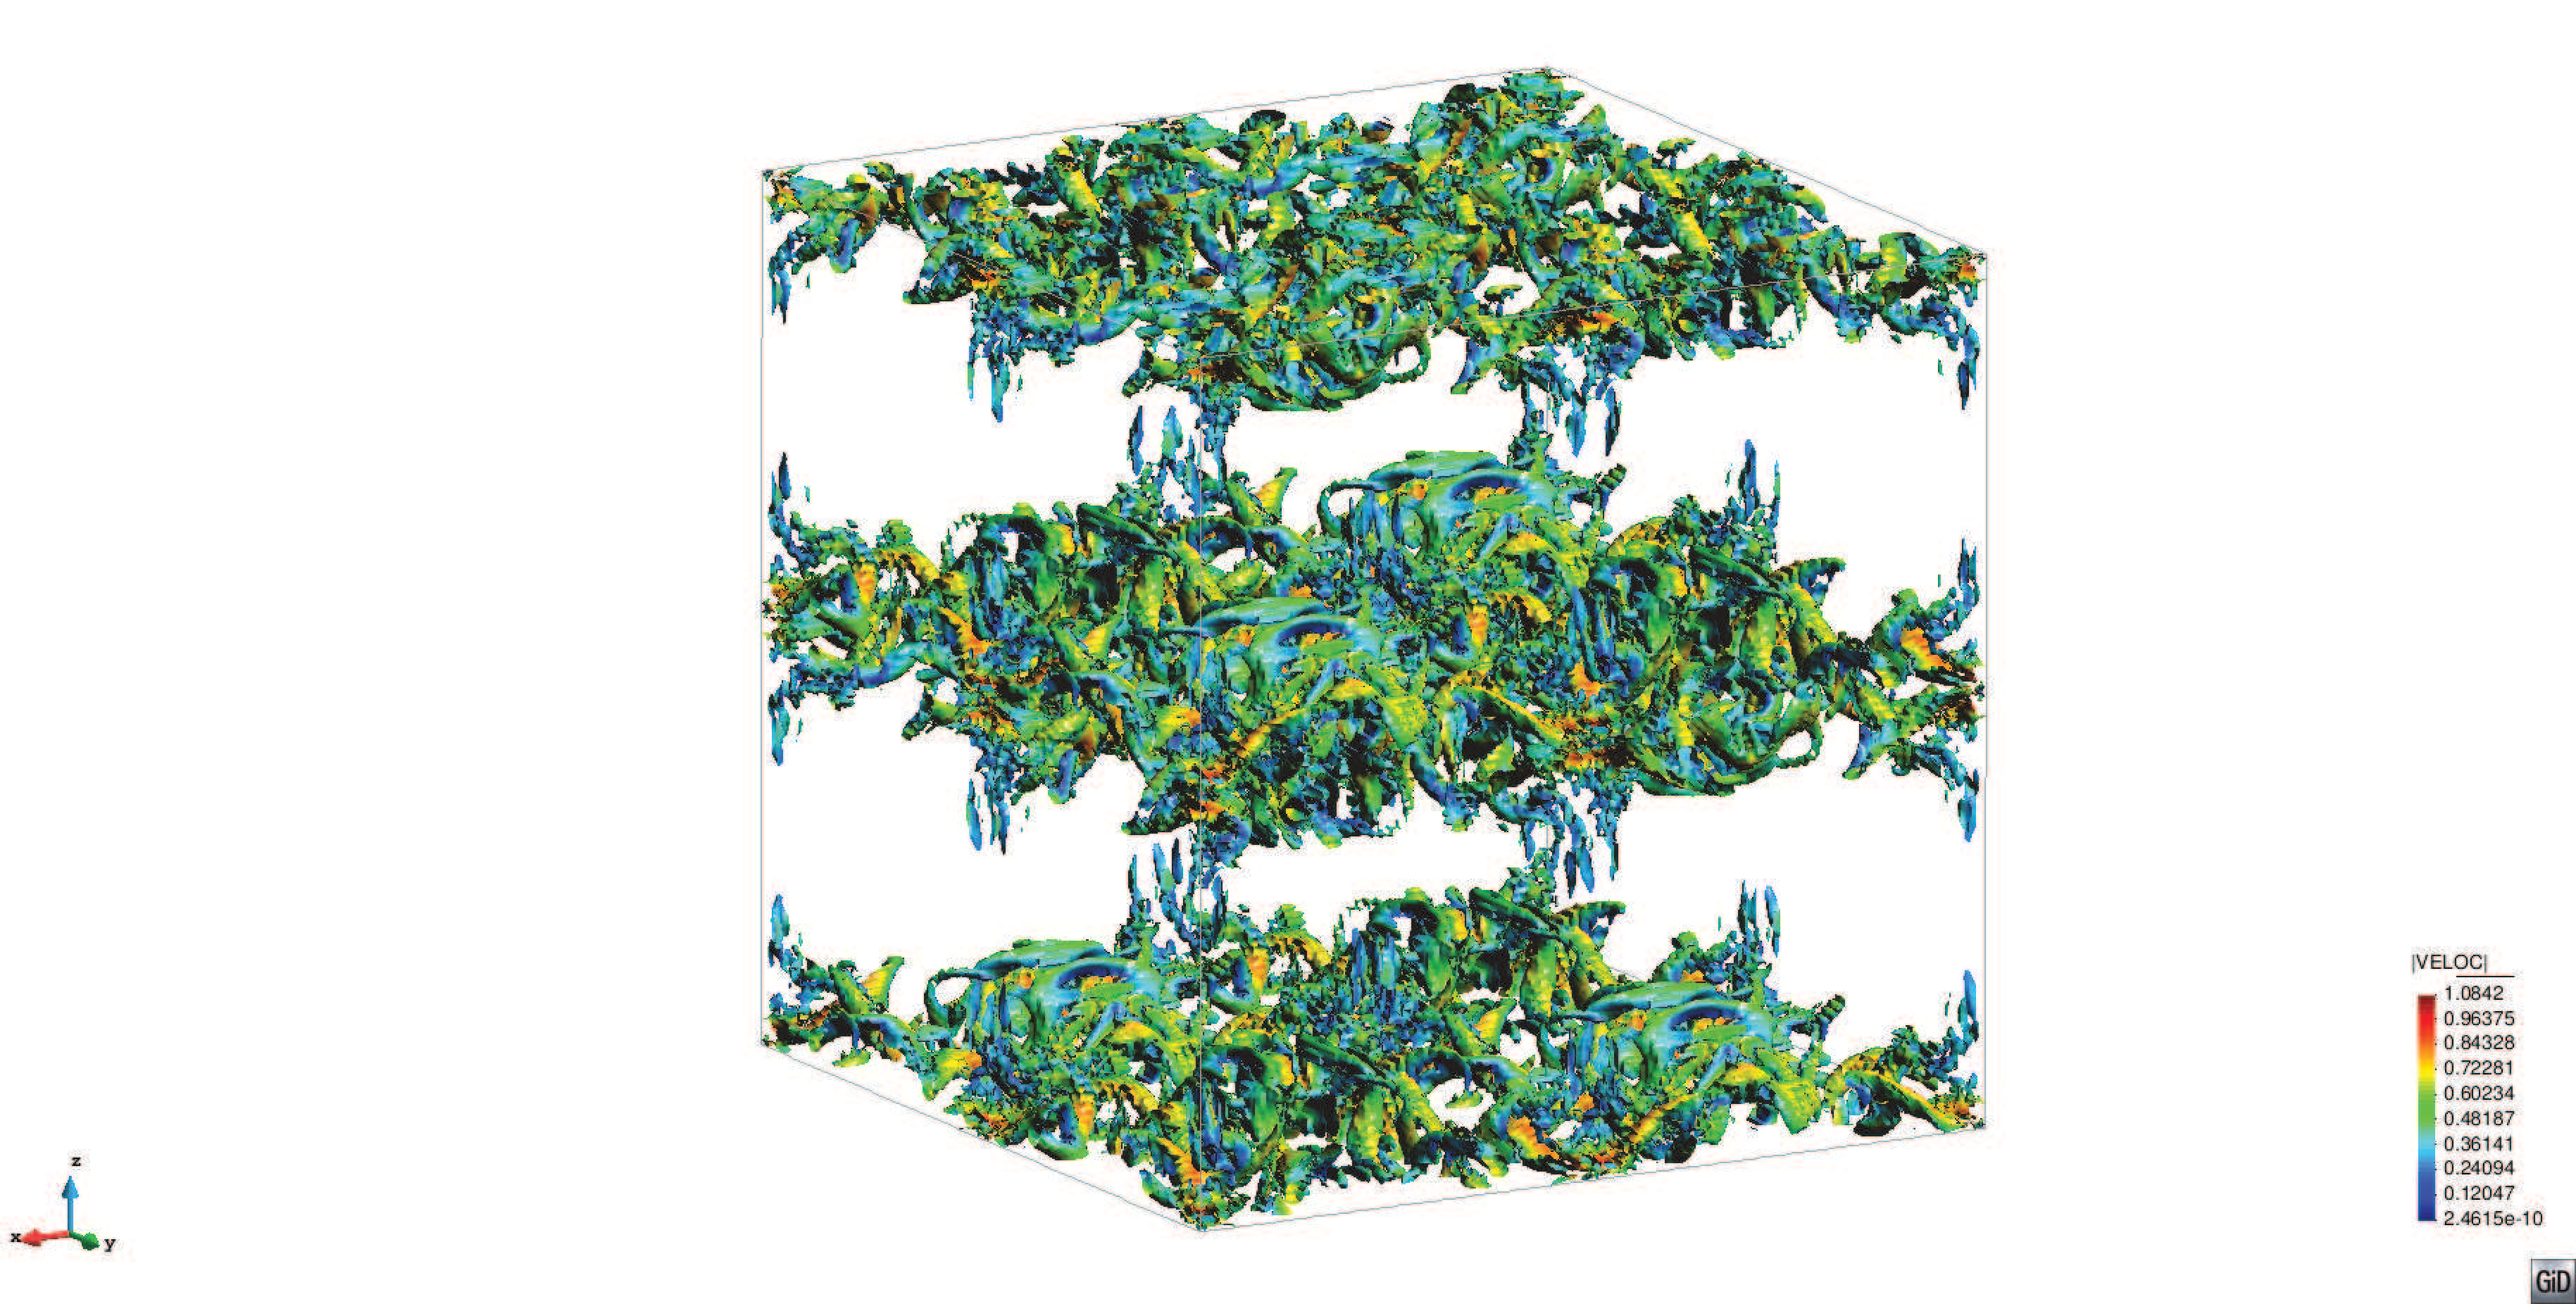
\includegraphics[width=1.0\textwidth]{Figures/isovorti_veloc_6}}{Movies/TGV.avi}
%\includemedia[activate=onclick,width=1.0\textwidth]{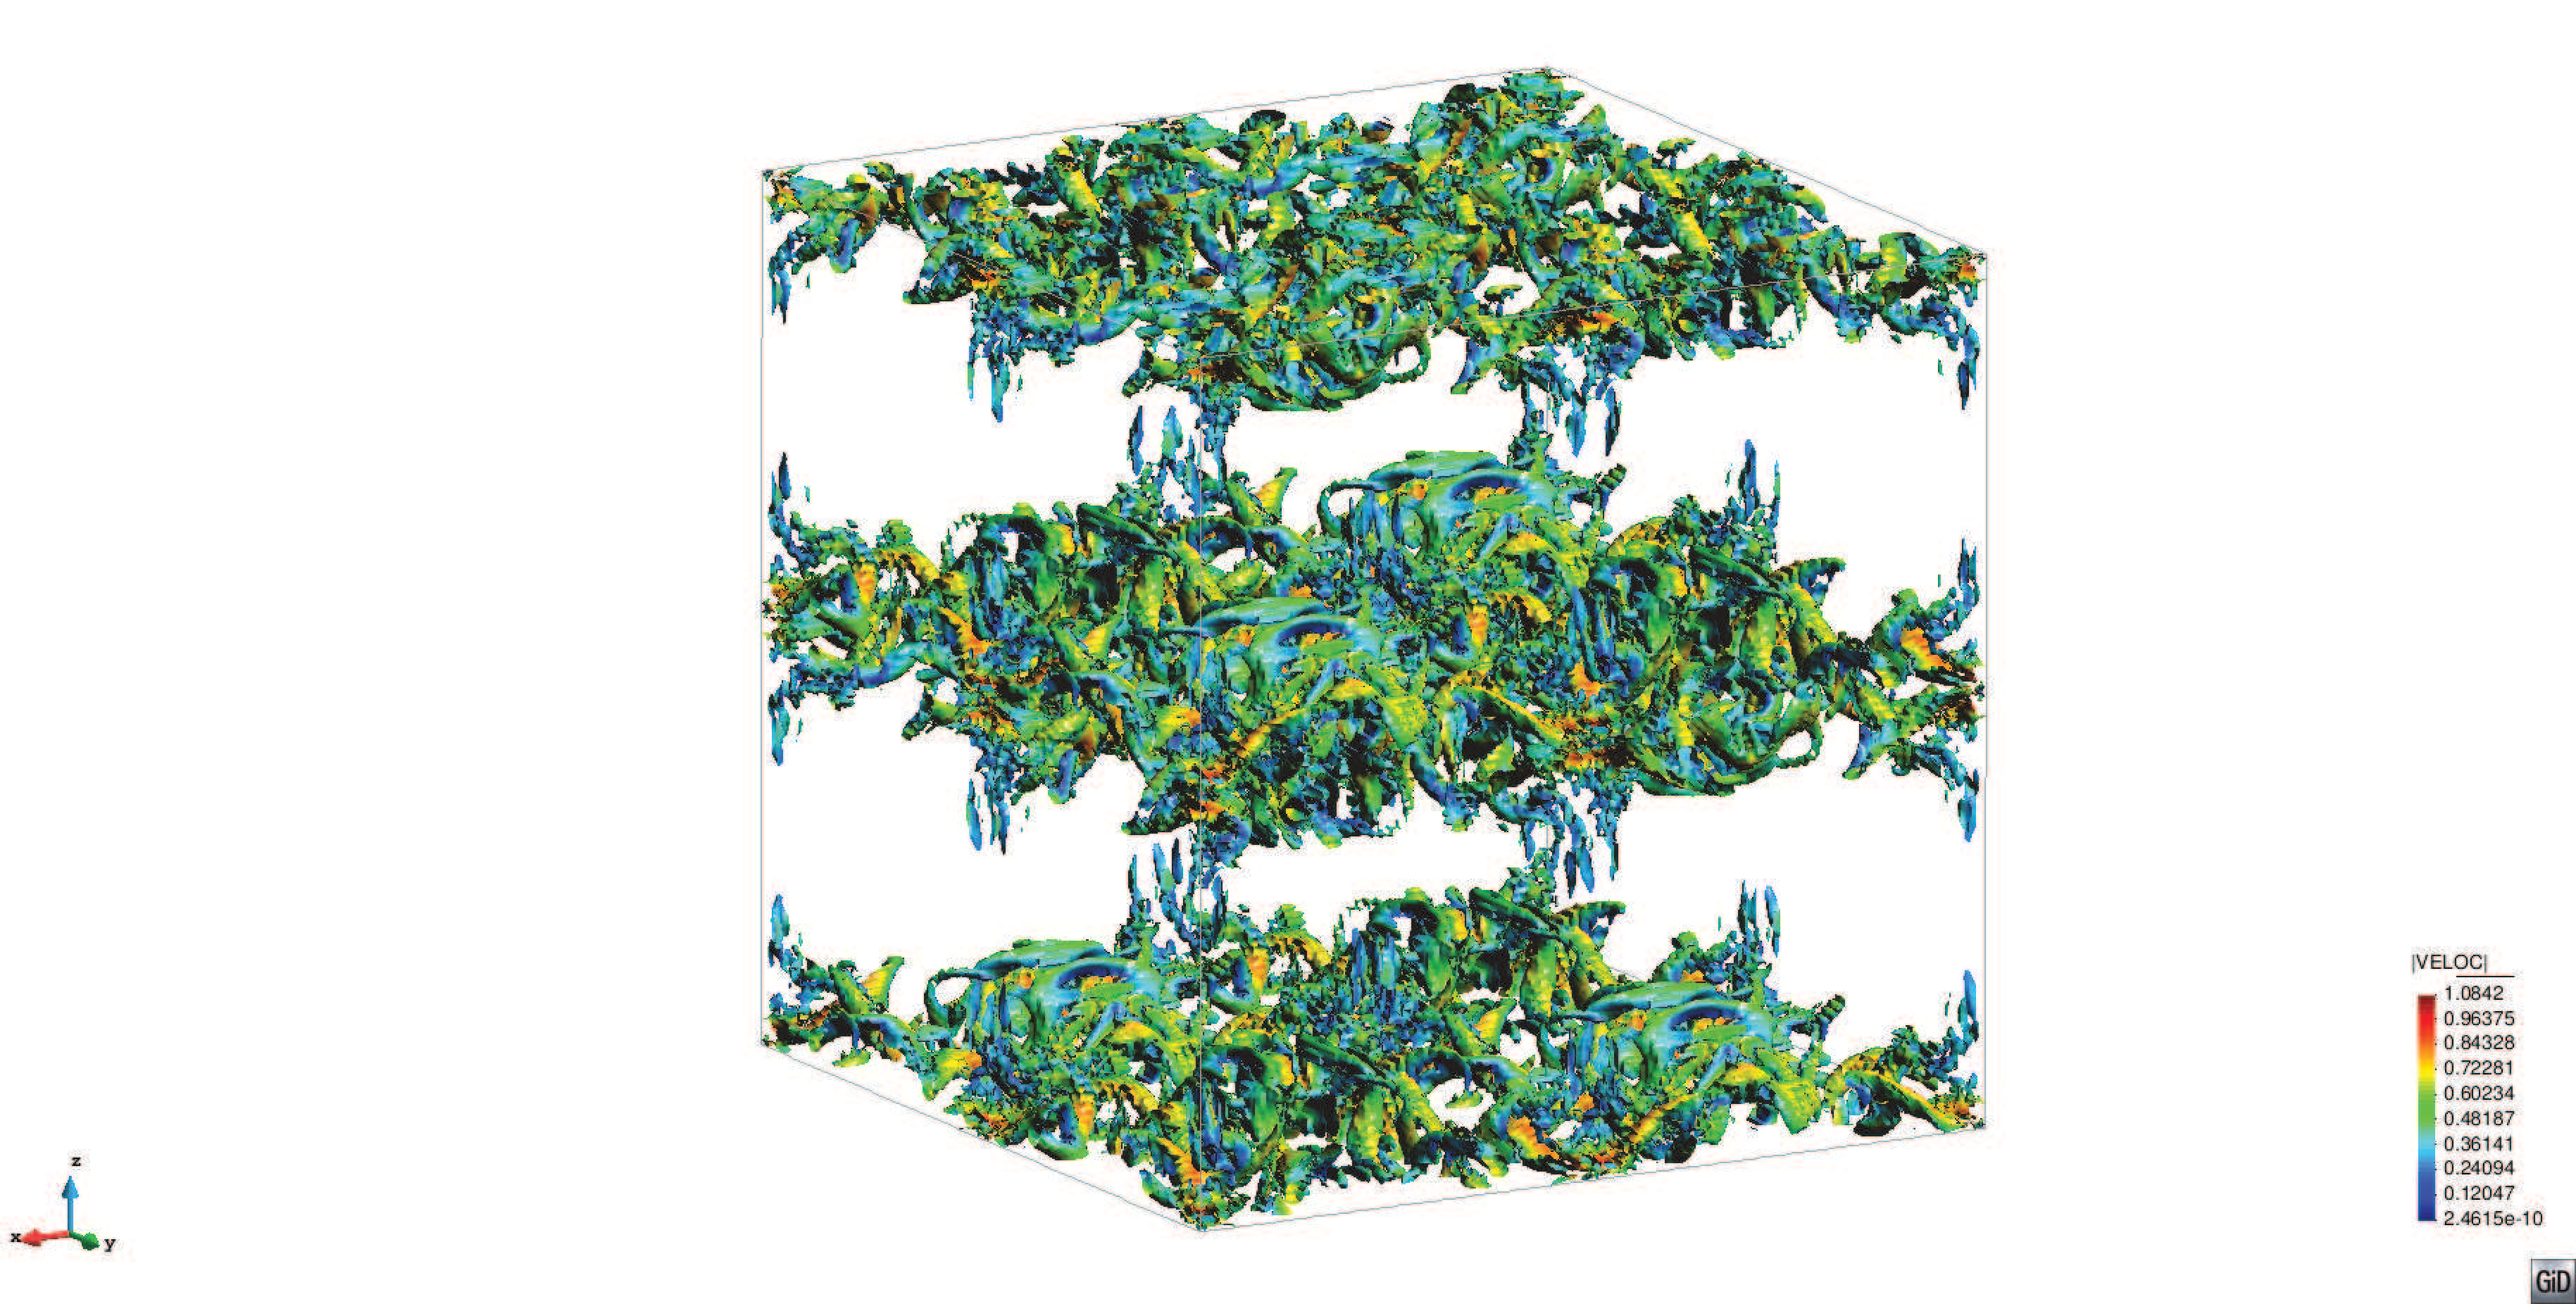
\includegraphics[width=1.0\textwidth]{Figures/isovorti_veloc_6}}{Movies/TGV.flv}
  \caption{Velocity isosurface}
 \end{figure} }
\end{frame}
%----------------------------------------------------------------------------------------
\begin{frame}
 \frametitle{TGV {\small Taylor-Green Vortex flow}}
 \textbf{Energy dissipation rate (refinement):}
 \vspace*{-1.0cm}
 \begin{columns}
   \begin{column}{0.5\textwidth}
   \begin{figure}
     \centering	
     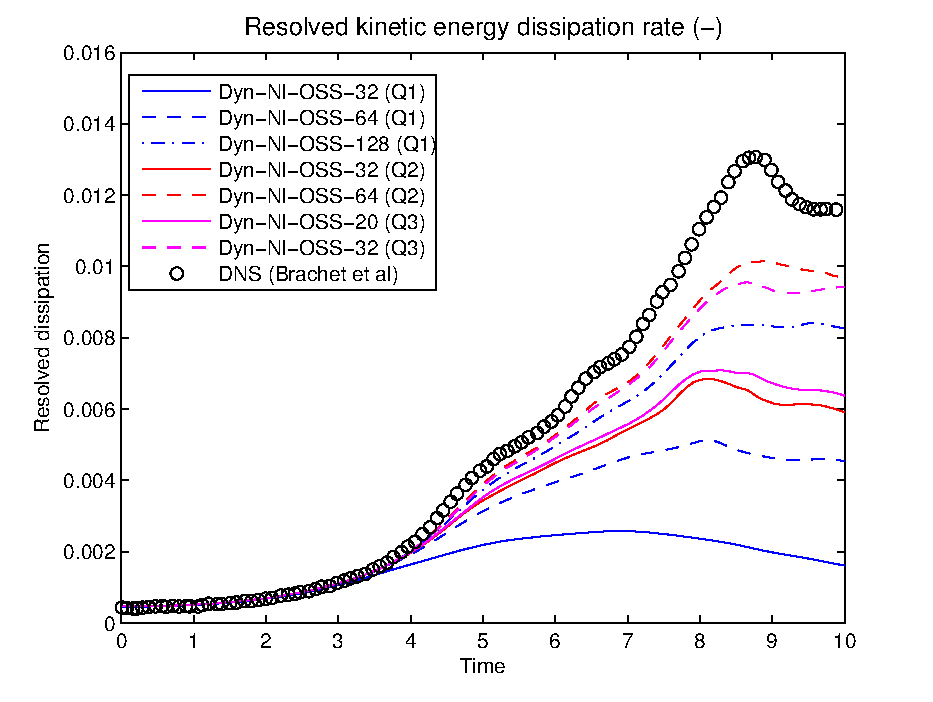
\includegraphics[width=1.1\textwidth]{Figures/ens_hp_10_new_resolved.pdf}
     \vspace*{-0.8cm}
     \caption{Resolved scales}
   \end{figure}
   \end{column}
   \begin{column}{0.5\textwidth}
   \begin{figure}
     \centering	
     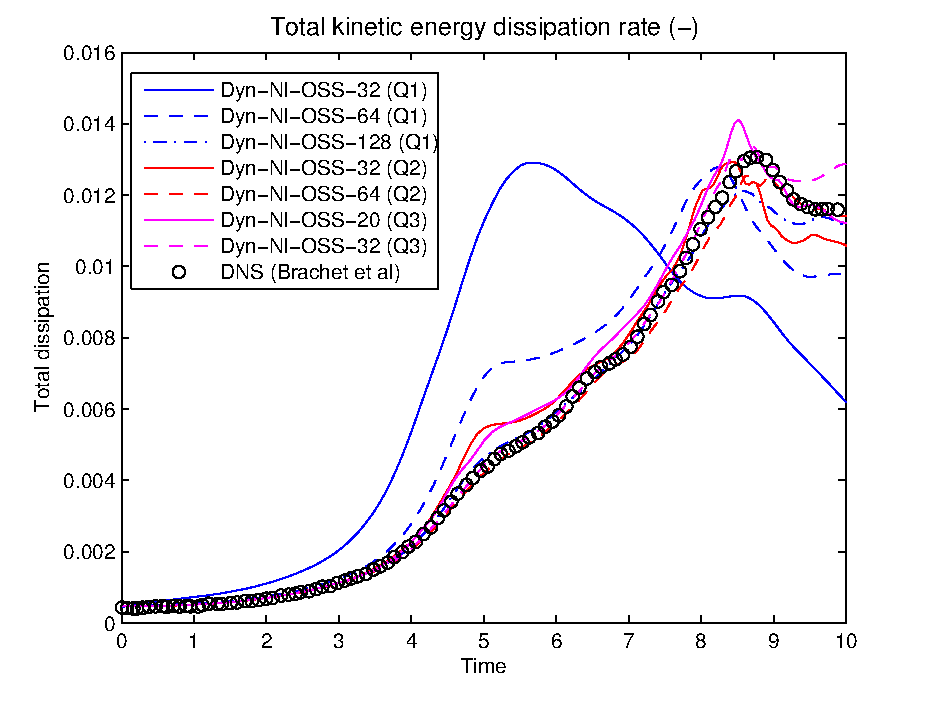
\includegraphics[width=1.1\textwidth]{Figures/ens_hp_10_new_total.pdf}
     \vspace*{-0.8cm}
     \caption{Total}
   \end{figure}
   \end{column}
 \end{columns}
 \begin{overlayarea}{\textwidth}{1.5cm}
 \only<2->{
 \vspace*{-0.3cm}
 \begin{itemize}
  	\item \alert<2>{Good agreement with the DNS} taking account the subscales
  	\only<3->{\item \alert<3>{More accurate results increasing the order} of approximation}
  \end{itemize}}
  \end{overlayarea}
\end{frame}
%----------------------------------------------------------------------------------------
\addtocounter{framenumber}{-1}
\begin{frame}
 \frametitle{TGV {\small Taylor-Green Vortex flow}}
 \vfill
 {\large
 \begin{itemize}
 	\item All results until now are compared against \textbf{DNS}
 \end{itemize}
 \vspace*{0.5cm}
  \begin{itemize}
  	\item Are our methods comparable with \textbf{LES} models?
 \end{itemize}}
 \vfill
\end{frame}
%----------------------------------------------------------------------------------------
\begin{frame}
 \frametitle{TGV {\small Taylor-Green Vortex flow}}
 \textbf{Energy dissipation rate (against LES model):}
 \vspace*{-1.0cm}
 \begin{columns}
   \begin{column}{0.5\textwidth}
   \begin{figure}
     \centering	
     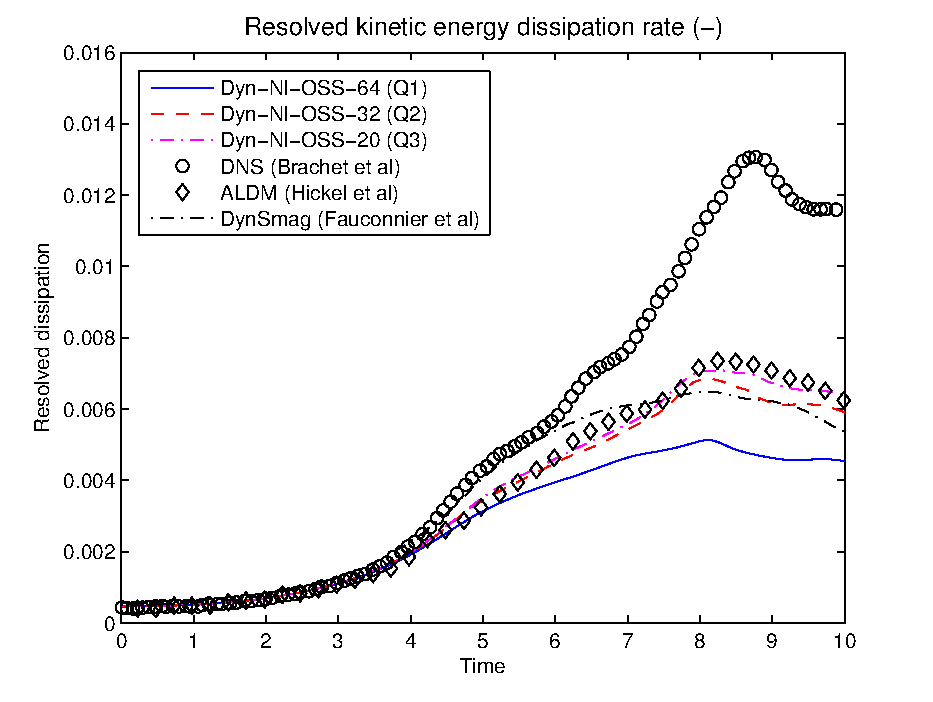
\includegraphics[width=1.1\textwidth]{Figures/ens_64dofs_dynsmag_resolved.pdf}
     \vspace*{-0.8cm}
     \caption{Resolved scales}
   \end{figure}
   \end{column}
   \begin{column}{0.5\textwidth}
   \begin{figure}
     \centering	
     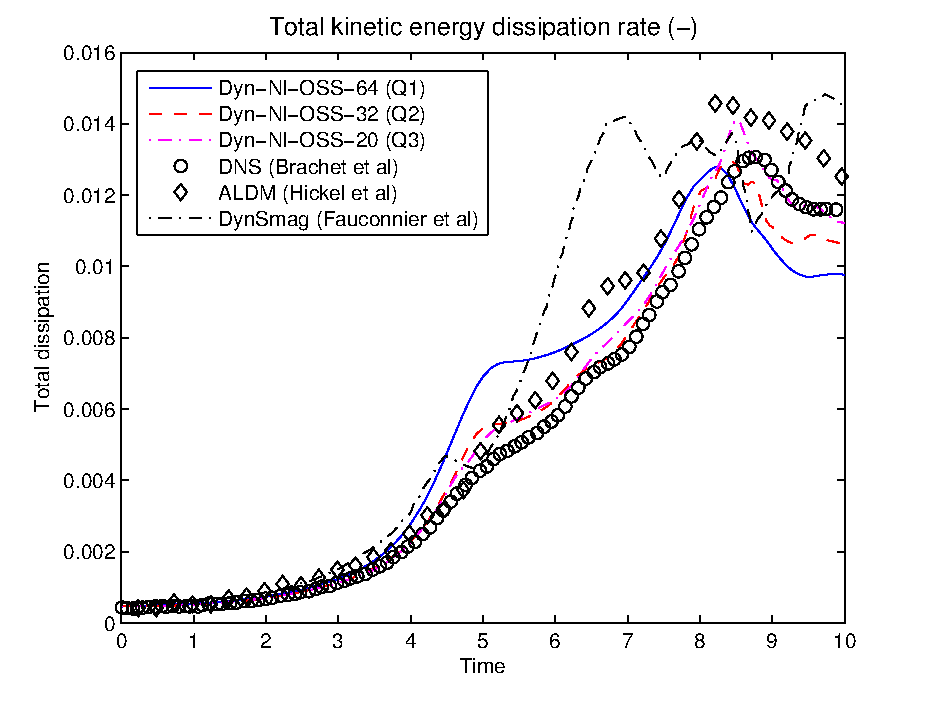
\includegraphics[width=1.1\textwidth]{Figures/ens_64dofs_dynsmag_total.pdf}
     \vspace*{-0.8cm}
     \caption{Total}
   \end{figure}
   \end{column}
 \end{columns}
 \begin{overlayarea}{\textwidth}{1.5cm}
  \only<2->{
  \vspace*{-0.3cm}
 \begin{itemize}
  	\item \alert<2>{Good agreement with the LES models} on resolved scales
  	\only<3->{\item \alert<3>{Better results than LES models} adding subscales counterpart}
  \end{itemize}}
  \end{overlayarea}
\end{frame}